\PassOptionsToPackage{usenames,dvipsnames}{xcolor}
\documentclass[tikz,border=2]{standalone}
\usepackage{amssymb}
\usepackage{enumerate}
\usepackage{mathtools} % contains amsmath which comes with align
\usepackage{amsthm}
\usepackage{graphicx}
\usepackage{microtype} % some compression
\usepackage[skins]{tcolorbox}
%%%%%%%%%%
% brown blue red
\definecolor{LightBlue}{HTML}{C7DFE3}
\definecolor{DarkBlue}{HTML}{72AFB6}
\definecolor{DarkBrown}{HTML}{D2BE89}
\definecolor{LightBrown}{HTML}{F4ECDF}
\definecolor{Grey}{HTML}{A7A195}
\definecolor{Red}{HTML}{CA6C2E}
%%
\def\labelitemi{\textcolor{gray}{\tiny{$\blacksquare$}}}
%%
\usetikzlibrary{shadows,arrows,shapes,trees,positioning,calc,backgrounds,
fit,automata,decorations.markings,
decorations.pathreplacing,decorations.pathmorphing}
%%%%%%%%%%%%%%%%%%%%%%%
\begin{document}
\begin{tikzpicture}[
      text width=1.5cm,
      align=center,
   node distance=3cm,
   grow=down,
   level 1/.style={sibling distance=3cm},
   level 2/.style={sibling distance=2cm},
   edge from parent/.style={draw,edge from parent fork down},
]
\node {Data sets \& APIs}
child {node[level distance=.5cm] {Spatial}
   child {node {GEO data}}
   child {node (oc) [yshift=-.1cm] {
\includegraphics[width=2cm]{aux/opencities.png}}}
}
child {node [yshift=-2cm]{Surveys}
   child {node (dhs){
\includegraphics[width=3cm]{aux/DHSProgram.png}}}
   child {node (ftf) [yshift=-1cm]{
\includegraphics[width=3cm]{aux/FtF.jpeg}}}
   child {node (ffp){Food for Peace}} %%{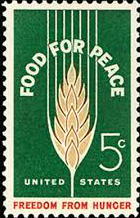
\includegraphics[width=1.2cm]{ffp.png}}}
   child {node (barometer) [yshift=-1.2cm]
      {
\includegraphics[width=2.5cm]{aux/americas_barometer.jpeg}}}
   child {node {Commuter surveys}}
   child {node [yshift=-1.2cm] {Program specific surveys}}
}
child {node {Experimental data}}
child {node {Commodity flow}
   child {node [yshift=0cm]
      {PEPFAR 
\includegraphics[width=1cm]{aux/pepfar-logo-seal.png}}}
}
;
\end{tikzpicture}
\end{document}
